% ============================================================
% Part 2 — Challenge Corner
% Hard and olympiad-style problems:
%   proving identities involving roots, geometry via polynomial
%   techniques, constructing polynomials from constraints,
%   extension/competition-level questions
% ============================================================

\begin{problem}[The Alternating Roots of $e^x$]
Let
\[
P_n(x)=\sum_{k=0}^{n}\frac{x^k}{k!}
\]
be the $n$th Maclaurin polynomial for $e^x$.
\begin{enumerate}[label=(\roman*)]
\item Assuming that for some even integer $2k$, the polynomial $P_{2k}(x)>0$ for all real $x$, prove that $P_{2k+1}(x)=0$ has exactly one real root.
\item Let $\alpha$ be the unique real root of $P_{2k+1}(x)=0$. By finding the global minimum of $P_{2k+2}(x)$, prove that $P_{2k+2}(x)>0$ for all real $x$.
\item Hence deduce the number of real roots of $P_n(x)=0$ when $n$ is even, and when $n$ is odd.
\end{enumerate}
\end{problem}

\begin{hintbox}
Use
\[
P_n'(x)=P_{n-1}(x)
\]
and
\[
P_n(x)=P_{n-1}(x)+\frac{x^n}{n!}.
\]
\end{hintbox}

\begin{solution}
Use
\[
P_n'(x)=P_{n-1}(x).
\]

\textbf{(i)} If $P_{2k}(x)>0$ for all real $x$, then
\[
P_{2k+1}'(x)=P_{2k}(x)>0,
\]
so $P_{2k+1}$ is strictly increasing. Since it has odd degree,
\[
P_{2k+1}(x)\to -\infty \text{ as }x\to -\infty,\qquad
P_{2k+1}(x)\to \infty \text{ as }x\to \infty.
\]
Hence $P_{2k+1}(x)=0$ has exactly one real root.

\textbf{(ii)} Let that root be $\alpha$. Then
\[
P_{2k+2}'(x)=P_{2k+1}(x),
\]
so $x=\alpha$ is the only stationary point of $P_{2k+2}$, hence its global minimum.
Now
\[
P_{2k+2}(x)=P_{2k+1}(x)+\frac{x^{2k+2}}{(2k+2)!},
\]
so
\[
P_{2k+2}(\alpha)=\frac{\alpha^{2k+2}}{(2k+2)!}>0
\]
because $P_{2k+1}(\alpha)=0$, $\alpha\ne0$, and $2k+2$ is even.
Thus
\[
P_{2k+2}(x)>0
\]
for all real $x$.

\textbf{(iii)} Starting from $P_0(x)=1>0$, parts (i) and (ii) give an induction chain:
\[
\boxed{P_n(x)=0\text{ has no real roots when }n\text{ is even,}}
\]
\[
\boxed{P_n(x)=0\text{ has exactly one real root when }n\text{ is odd.}}
\]
\end{solution}

\begin{takeaways}
\begin{itemize}[leftmargin=*]
\item The derivative relation $P_n'=P_{n-1}$ links consecutive Maclaurin polynomials.
\item Evaluating the even polynomial at the odd polynomial’s root makes the summation collapse to one positive term.
\item This creates an induction pattern: even cases have no real roots, odd cases have exactly one.
\end{itemize}
\end{takeaways}

\begin{problem}[The Geometric Solution of the Quartic]
\textbf{Historical Context}

Before the development of symbolic algebra in the $16$th century, solving cubic and quartic equations was one of the great challenges of mathematics. While quadratic equations could be handled geometrically, higher-degree equations seemed much harder.

\textbf{Omar Khayyam} ($1048$--$1131$), the Persian mathematician, astronomer, and poet, gave a remarkable geometric approach: instead of searching for a symbolic formula, he represented roots as intersection points of conic sections.

The following problem recreates that idea using modern Cartesian coordinates.

\medskip
\noindent Consider the rectangular hyperbola
\[
\mathcal H:\ y=\frac{1}{x},\qquad x\ne 0,
\]
and the circle
\[
\mathcal C:\ (x-c)^2+y^2=c^2,
\]
where $c>0$.

\begin{enumerate}[label=(\roman*)]
\item By substituting the equation of the hyperbola into the equation of the circle, show that the $x$-coordinates of the intersection points are the roots of
\[
P(x)=x^4-2cx^3+1.
\]
\item Use $P'(x)$ to show that if
\[
c>\sqrt[4]{\frac{16}{27}},
\]
then $P(x)$ has exactly two distinct real roots. Interpret this geometrically.
\item Let the four roots be $\alpha,\beta,\gamma,\delta$. Find the value of
\[
\alpha\beta\gamma\delta.
\]
\item \textbf{The Khayyam Challenge:} For what value of $c$ does the circle become tangent to the hyperbola? Justify your answer using multiplicity of roots.
\end{enumerate}
\end{problem}

\begin{center}
\begin{tikzpicture}
\begin{axis}[
  axis lines=middle,
  xmin=-1.2,xmax=2.4,
  ymin=-1.4,ymax=1.4,
  samples=300,
  width=0.68\linewidth,
  height=6.1cm,
  xtick=\empty,
  ytick=\empty,
  xlabel={$x$},
  ylabel={$y$},
  enlargelimits=false,
  axis equal image=true
]
\addplot[thick,bookpurple,domain=-1.2:-0.28] {1/x};
\addplot[thick,bookpurple,domain=0.28:2.4] {1/x};
\addplot[thick,blue!70!black,domain=0:360,samples=240] ({0.5 + 0.5*cos(x)},{0.5*sin(x)});
\addplot[thick,orange!90!black,domain=0:360,samples=240] ({(16/27)^(1.0/4.0) + (16/27)^(1.0/4.0)*cos(x)},{(16/27)^(1.0/4.0)*sin(x)});
\addplot[thick,red!75!black,domain=0:360,samples=240] ({1 + cos(x)},{sin(x)});
\end{axis}
\end{tikzpicture}

\small Hyperbola $\mathcal H$ in purple. Circles shown for $c=\frac12$ (blue), $c=\sqrt[4]{\frac{16}{27}}\approx 0.87738$ (orange), and $c=1$ (red).
\end{center}

\begin{center}
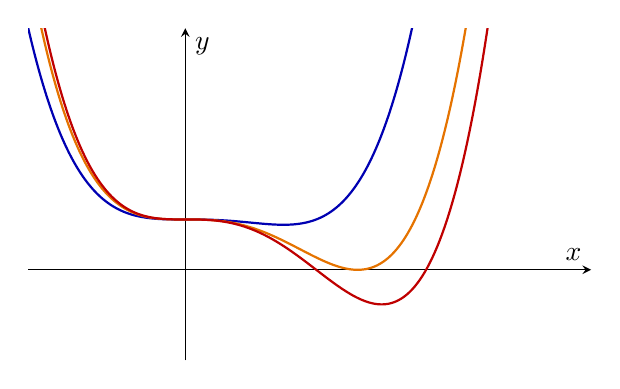
\begin{tikzpicture}
\begin{axis}[
  axis lines=middle,
  xmin=-1.2,xmax=3.1,
  ymin=-1.8,ymax=4.8,
  samples=400,
  width=0.72\linewidth,
  height=5.8cm,
  xtick=\empty,
  ytick=\empty,
  xlabel={$x$},
  ylabel={$y$},
  enlargelimits=false
]
\addplot[thick,blue!70!black,domain=-1.2:3.1]{x^4 - x^3 + 1};
\addplot[thick,orange!90!black,domain=-1.2:3.1]{x^4 - 2*((16/27)^(1.0/4.0))*x^3 + 1};
\addplot[thick,red!75!black,domain=-1.2:3.1]{x^4 - 2*x^3 + 1};
\end{axis}
\end{tikzpicture}

\small Quartics $P(x)=x^4-2cx^3+1$ for $c=\frac12$ (blue), $c=\sqrt[4]{\frac{16}{27}}\approx 0.87738$ (orange), and $c=1$ (red).
\end{center}

\begin{hintbox}
For tangency, the quartic must have a repeated real root. So solve $P(x)=0$ and $P'(x)=0$ together.
\end{hintbox}

\begin{solution}
\textbf{(i)} Substitute $y=\frac1x$ into the circle:
\[
(x-c)^2+\frac1{x^2}=c^2.
\]
\[
x^2-2cx+\frac1{x^2}=0
\]
and hence
\[
\boxed{x^4-2cx^3+1=0.}
\]

\textbf{(ii)} For
\[
P(x)=x^4-2cx^3+1,
\]
\[
P'(x)=4x^3-6cx^2=2x^2(2x-3c).
\]
So the relevant stationary point is $x=\frac{3c}{2}$. Also
\[
P\!\left(\frac{3c}{2}\right)=\left(\frac{3c}{2}\right)^4-2c\left(\frac{3c}{2}\right)^3+1
=1-\frac{27c^4}{16}.
\]
\[
\text{If }c>\sqrt[4]{\frac{16}{27}},\text{ then }P\!\left(\frac{3c}{2}\right)<0.
\]
Since $P(x)\to+\infty$ as $x\to\pm\infty$, the quartic crosses the $x$-axis exactly twice. Therefore it has exactly two distinct real roots, so geometrically the circle and hyperbola meet at exactly two real points.

\textbf{(iii)} By Vieta,
\[
\alpha\beta\gamma\delta=\frac{1}{1}=\boxed{1}.
\]

\textbf{(iv)} Tangency occurs when the quartic has a repeated real root. So solve
\[
P(x)=0,\qquad P'(x)=0.
\]
From $P'(x)=0$, the repeated root must occur at $x=\frac{3c}{2}$. So
\[
P\!\left(\frac{3c}{2}\right)=0
\Rightarrow 1-\frac{27c^4}{16}=0.
\]
\[
\boxed{c=\sqrt[4]{\frac{16}{27}}=\frac{2}{\sqrt[4]{27}}.}
\]
\end{solution}

\begin{takeaways}
\begin{itemize}[leftmargin=*]
\item Intersections of conics can encode polynomial roots geometrically.
\item Clearing denominators can convert a geometry problem into a quartic equation.
\item Tangency corresponds to a repeated root, so the equations $P(x)=0$ and $P'(x)=0$ should be solved together.
\end{itemize}
\end{takeaways}

\begin{problem}[A Cubic with a Double Root]
The equation
\[
x^3-5x^2+mx-3=0
\]
has a double root. Find $m$.
\end{problem}

\begin{hintbox}
Use $P(r)=0$ and $P'(r)=0$ for a double root $r$.
\end{hintbox}

\begin{solution}
Let
\[
P(x)=x^3-5x^2+mx-3.
\]
If $r$ is a double root, then
\[
P(r)=0,\qquad P'(r)=0.
\]
Since
\[
P'(x)=3x^2-10x+m,
\]
we have
\[
m=10r-3r^2.
\]
Substitute into $P(r)=0$:
\[
r^3-5r^2+r(10r-3r^2)-3=0.
\]
So
\[
2r^3-5r^2+3=0.
\]
Factor:
\[
(r-1)(2r^2-3r-3)=0.
\]
The easy integer root is $r=1$, so
\[
\boxed{m=10(1)-3(1)^2=7.}
\]
\[
\text{Indeed, }x^3-5x^2+7x-3=(x-1)^2(x-3).
\]
\end{solution}

\begin{takeaways}
\begin{itemize}[leftmargin=*]
\item Repeated-root parameter questions naturally produce a system in $r$ and the parameter.
\item A well-chosen repeated root often gives a simple integer value for the parameter.
\end{itemize}
\end{takeaways}

\begin{problem}[No Real Roots via Global Minimum]
Prove that the polynomial below has no real roots:
\[
P(x) = \frac{x^8}{8} + \frac{x^7}{7} + \frac{x^6}{6} + \frac{x^5}{5} + \frac{x^4}{4} + \frac{x^3}{3} + \frac{x^2}{2} + x + \frac{11}{16}
\]
\end{problem}

\begin{hintbox}
\begin{itemize}[leftmargin=*]
\item Differentiate $P(x)$ to find its stationary points. Do you recognize the geometric progression in $P'(x)$? Rewrite it using the sum formula.
\item Find the exact $x$-coordinate of the only real turning point.
\item Evaluate $P(x)$ at this turning point to find the global minimum. If the lowest possible point on an even-degree polynomial sits above the $x$-axis, what does that mean for its roots?
\end{itemize}
\end{hintbox}

\begin{solution}
\textbf{1. Find the derivative to locate stationary points:}\\
\[
P'(x) = x^7 + x^6 + x^5 + x^4 + x^3 + x^2 + x + 1
\]
Recognizing this as a geometric series with common ratio $x$, we can rewrite it (for $x \neq 1$) as:
\[
P'(x) = \frac{x^8 - 1}{x - 1}
\]

\textbf{2. Solve $P'(x) = 0$ for critical points:}\\
\[
\frac{x^8 - 1}{x - 1} = 0 \implies x^8 - 1 = 0 \quad (\text{where } x \neq 1)
\]
The real solutions to $x^8 = 1$ are $x = 1$ and $x = -1$.
Since $x \neq 1$ (which makes the denominator zero), our only valid stationary point is \textbf{$x = -1$}.

\textbf{3. Determine the nature of the stationary point:}\\
Analyze the sign of $P'(x)$ around $x = -1$:
\begin{itemize}[leftmargin=*]
\item For $x < -1$ (e.g., $x = -2$): $P'(-2) = -85 < 0$ (Decreasing)
\item For $-1 < x < 1$ (e.g., $x = 0$): $P'(0) = 1 > 0$ (Increasing)
\end{itemize}
Since the curve changes from decreasing to increasing, $x = -1$ is a local minimum. Because it is the \emph{only} turning point and the polynomial has an even degree with a positive leading coefficient, it is the \textbf{global minimum}.

\textbf{4. Evaluate the global minimum:}\\
Substitute $x = -1$ into the original polynomial:
\[
P(-1) = \frac{(-1)^8}{8} + \frac{(-1)^7}{7} + \dots + \frac{(-1)^2}{2} + (-1) + \frac{11}{16}
\]
\[
P(-1) = \frac{1}{8} - \frac{1}{7} + \frac{1}{6} - \frac{1}{5} + \frac{1}{4} - \frac{1}{3} + \frac{1}{2} - 1 + \frac{11}{16}
\]
Find a common denominator for the first eight fraction terms ($840$):
\[
P(-1) = \left( \frac{105 - 120 + 140 - 168 + 210 - 280 + 420 - 840}{840} \right) + \frac{11}{16}
\]
\[
P(-1) = -\frac{533}{840} + \frac{11}{16}
\]
Find a common denominator ($1680$) to add these final fractions:
\[
P(-1) = -\frac{1066}{1680} + \frac{1155}{1680} = \mathbf{\frac{89}{1680}}
\]

\textbf{Conclusion:}\\
Since $\frac{89}{1680} > 0$, the absolute lowest point of the curve is strictly above the $x$-axis. Therefore, $P(x) > 0$ for all real $x$, meaning the equation $P(x) = 0$ has \textbf{no real roots}.
\end{solution}

\begin{takeaways}
\begin{itemize}[leftmargin=*]
\item \textbf{Calculus as a Root-Finding Tool:} You do not need to solve an equation to prove it has no solutions. Proving the global minimum is strictly positive is a powerful Extension 1 technique.
\item \textbf{The Geometric Polynomial:} The expression $x^n + x^{n-1} + \dots + x + 1$ appears frequently. Immediately recognizing it as $\frac{x^{n+1}-1}{x-1}$ saves time and avoids messy factor-by-grouping methods.
\end{itemize}
\end{takeaways}
